%\documentclass[a4paper]{article}
\documentclass[10pt]{article}
\usepackage{comment} % enables the use of multi-line comments (\ifx \fi) 
\usepackage{lipsum} %This package just generates Lorem Ipsum filler text. 
\usepackage{fullpage} % changes the margin
\usepackage{graphicx}
\usepackage{hyperref}

\hypersetup{
    colorlinks=true, 
    urlcolor=cyan,
}

\begin{document}
\noindent
\large\textbf{Introduction to Data Science: Homework 3} \hfill STAT1021, Spring 2018
\\
Guest lecturer: Tzu-Chi Yen
\hfill Due: May 1st 23:59

\begin{enumerate}
	%	
	% Problem 1
	%
	\item{(18 pts total) Give \textbf{one} real-life example of each of the following types of networks; then, {\it briefly} describe \textbf{one} empirical technique that could be used to measure the structure of each of the following networks (i.e., to fully determine the positions of all the edges), and \textbf{one} phenomenon regarding the network that you are interested in which network analysis methods may help to understand:
	\begin{enumerate}
	\item{(3 pts) An acyclic (or approximately acyclic) directed network}
	\item{(3 pts) A cyclic directed network}
	\item{(3 pts) A tree (or approximate tree)}
	\item{(3 pts) A planar (or approximately planar) network}
	\item{(3 pts) A bipartite network}
	\item{(3 pts) A temporal network (or sequence of edges)
	}
	\end{enumerate}
	}
	% 
	% Problem 2
	%
	\item{(14 pts total) Consider the following three networks:
		\begin{figure}[ht]
		\centering
		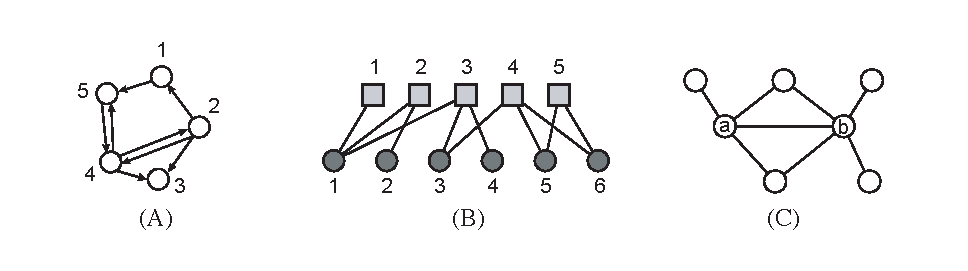
\includegraphics[width=0.9\textwidth]{fig-1.pdf}	
		\end{figure}
		\begin{enumerate}
			\item{(3 pts) Give the adjacency matrix for network (A).}
			\item{(3 pts) Give adjacency list for network (A).}	
			\item{(5 pts) Give adjacency matrices for both one-mode projections of network (B).}
%			\item{(3 pts) Find a 2-core in network (C).}
			\item{(3 pts) What is the cosine similarity of vertices \texttt{a} and \texttt{b} in network (C)?}
		\end{enumerate}
	}
	%
	% Problem 3
	%
	\item{(46 pts total) In this question, we will investigate several properties of a social network (and build a recommendation system for it!) by analyzing the results of the in-class social network questionnaire, which you may download from here:
	
	\begin{center}
		\url{http://wiki.junipertcy.info/images/5/56/In-class_network.txt}
	\end{center}
	
	To complete this homework problem you'll need to use Python and the \texttt{networkx} library. And you have to submit this part of your homework by sending a pull request on GitHub. So -- first things first, fork the following project into your GitHub repository:
	
	\begin{center}
		\url{https://github.com/junipertcy/networkie}
	\end{center}
	
	Note that the network is directed: person $P_1$ may know (nominate) person $P_2$ but not {\it vice versa}. For simplicity, let us define an undirected symmetrized network, in which there is an undirected edge between nodes $i$ and $j$ if there is a directed edge either from $i$ to $j$ or from $j$ to $i$. Let $A$ be the adjacency matrix of the simple graph.
	
	In order to analyze this network, you will need to load it into a graph analytic library as a functional data class. You may, of course, add each link one-by-one by hand, but it is often useful to write a {\it parser} that directly convert the text file into graph-library-friendly formats.
	\begin{enumerate}
		\item{(8 pts) Write a function that parses the \texttt{In-class\_network.txt} file to a \texttt{networkx} Graph object.} [{\it hint:} the function is in \texttt{networkie/gen/Custom.py}]
		\item{(10 pts, 2 pts each) Show common descriptive statistics for the network $A$, which are (i) the number of nodes $n$; (ii) the number of edges $e$; (iii) average degree $\langle k \rangle$; (iv) average path length $l$, and (v) the size of the largest connected component $n_G$.}
		\item{(8 pts) Most empirical networks are sparse. If the network is fully connected (i.e. it's a complete graph), compute its number of edges $e_{max}$. What is $e/e_{max}$?}
		\item{(8 pts) Write a function which outputs the vector \textbf{k}, as a Python list, whose elements are the degrees $k_i$ of vertex $i$. Use the `ID' key in the file as the index $i$ of the list. Plot the degree distribution in a separate \texttt{*.ipynb} file.} ({\it hint:} the function is in \texttt{networkie/utils/Measures.py})
%		\item{(5 pts) Write a function which outputs the matrix \textbf{N}, as a `numpy::ndarray', whose elements $N_{ij}$ is equal to the number of common neighbors of vertices i and j.}
		\item{(12 pts) In a social network, when there is a tie from $i$ to $j$ and also a tie from $j$ to $h$, if there is also a tie from $i$ to $h$, we call the three nodes form a {\it transitive triad} \footnote[1]{Empirical social networks are known to possess abundant triangles. In sociology, there has been much theorizing over the years about the structural properties of a social network which are manifested at the local level of dyads and triads. See chapter 3 from the book, "{\it Networks, Crowds, and Markets}": \url{http://bit.ly/2GGXcG9}}, or a {\it triangle}. Write a function that calculates the total number of triangles in the network $n_\Delta$. What is $n_\Delta$ for the data? (You get only 5 points if you directly call an existing API from a library.) [{\it hint:} the function is in \texttt{networkie/utils/Measures.py}]}
	\end{enumerate}
	%
	% Problem 4
	%	
	\item{(12 pts total) We have included new components in our {\it networkie} library! Our goal is not only to make it useful, but to attract people and persuade them that we are working on an interesting project. To make it easier for other people to participate in the project, we need a good documentation.
	\begin{enumerate}
		\item{(12 pts, 4 pts each) Write the {\it docstring} documentation for the functions that you write in problems (3-a, 3-d, and 3-e). If you are unable to complete any of the previous problems, you will still get the points by writing the documentation in an virtual function. Please follow the style convention of existing functions.}
	\end{enumerate}
	}
	%
	% Problem 5
	%
	\item{(10 pts total)
	A repository with unit tests prevents errors when the code grows. Unlike common software development practices in the industry, which usually have well-defined target of tests (e.g. user authentication, form value validation), it is not easy to define a good unit test for a scientific project. Nevertheless, we can still enforce constraints in the existing workflow by inserting an assertion in the code. This is a simple example of {\it defensive programming}, but effective.
	\begin{enumerate}
		\item{(6 pts) Construct a new unit test which asserts that $e = \frac{1}{2}\Sigma_i{k_i}$, using the function that you write in Problem 3-d. This ensures that the function is implemented correctly, no matter what network data we face (as long as it is simple).}
		\item{(4 pts) Update the \texttt{.travis.yml} file whenever necessary, commit and push the code to the remote repository. Make sure that you passed the test with the sample data (i.e. the karate club network).}
	\end{enumerate}	
	
	}
	%
	% Problem 6
	%
	\item{ (20 pts total, {\it extra credit}) Many social media systems, such as Facebook and Twitter, recommends people for users to follow based on the idea of triadic closure. This means, for a node $v_i$ in the social network $G = (V, E)$, we may connect it to {\it one} adjacent node $v_i^a \in V$, such that a new triangle is formed. With this construction, the number of {\it potential friends} $\| V_i \|$ varies from person to person. For an isolated node $v_\textsubscript{iso}$, $\| V_\textsubscript{iso} \| = 0$.
	
	\begin{enumerate}
		\item{(5 pts) Write a function which outputs the vector \textbf{r}, as a Python list of sets, whose element is the set of IDs, representing the collection potential ``friends'' $\lbrace v_i^a \rbrace$ of vertex $i$.}				
		
	\end{enumerate} 
	To build a recommendation system for the social network based on the number of common friends, we assume that a new friend can be recommended to someone if they have common friends. And $\textbf{r}$ tells us which persons to recommend for a particular user $i$. Regarding these potential edges, we could do further by assuming the more common friends the two non-friends share, the higher likelihood that they will make new friends. The degree vector in Prob. 3-d gives us a way to {\it rank} the importance of the edges. Hence, the best friend recommendation is the person with whom you have the largest number of mutual friends. We will implement this heuristic.
	\begin{enumerate}
		\item{(5 pts) Student ID 45 has only 2 friends, please suggest 3 new friends to her based on the top choices from the algorithm. }
		\item{(10 pts) If the mechanism of building new friendships follows the heuristic, the algorithm may help us {\it predict} new friendship edges. Let's do an experiment by randomly removing 5\% of the friendship edges, and virtually add the edges back one by one, adaptively, according to the ranked recommendation list, until the sparsified network has the same number of edges as the original network. Are the two networks similar? Discuss your result.\footnote[2]{At the end, you might find that there are {\it more} triads in the synthetic network. In other words, the algorithm has a tendency to promote triadic closure, and this complicates researchers' ability to use data to study social preferences. The ways that the goals of system designers can introduce patterns into data is called {\it algorithmic confounding}. See section 2.3.8 of the book, "{\it Bit by Bit}": \url{http://bit.ly/2GHv8CG}.}}
	\end{enumerate}
	
	}
	}
\end{enumerate}
\subsection*{Submit your homework}
All of your coding work should be submitted via a pull request to the {\it networkie} library on GitHub. The deliverables are listed in the following:

\begin{enumerate}
	\item{One PDF file, in the \texttt{/} directory (root directory), stating your answers to Problems 1 and 2. At the bottom of your PDF file, create a ``collaboration'' section, state which students or other people (besides the course staff) helped you with the assignment, or that no one did. Finally, rename the file as \texttt{\$YOUR\_STUDENT\_ID.pdf}.}
	\item{One Jupyter Notebook after you have finished the coding quizzes. Make sure the newly-written functions work adequately by calling the them in \texttt{/hw3.ipynb}.}
	\item{Complete the \texttt{/tests/test\_compute\_degrees.py}, file. Make sure that the unit test passes by running {\it pytest}.}
	\item{If you answered Prob. 6, add them to the repo.}
	\item{Stage all your awesome homework, push it to your remote repo, and see if Travis CI gives you a green pass sign. This is for Prob. 5-b.}
	\item{Send the author a pull request.}
\end{enumerate}

Now you are done! I hope you enjoyed the special lectures. Email me when you have questions. Good luck!


\end{document}
